\documentclass{article}

\usepackage{graphicx} %[pdftex] OR [dvips]
\usepackage{fullpage}
\usepackage{float}
\usepackage{titling}
\setlength{\droptitle}{-6em}

\newcommand{\ghcfile}[1]{\textsl{#1}}

\title{Implementing Backpack}

\begin{document}

\maketitle

The purpose of this document is to describe an implementation path
for Backpack~\cite{Kilpatrick:2014:BRH:2535838.2535884} in GHC\@.

We start off by outlining the current architecture of GHC, ghc-pkg and Cabal,
which constitute the existing packaging system.  We then state what our subgoals
are, since there are many similar sounding but different problems to solve.  Next,
we describe the ``probably correct'' implementation plan, and finish off with
some open design questions.  This is intended to be an evolving design document,
so please contribute!

\section{Current packaging architecture}

The overall architecture is described in Figure~\ref{fig:arch} (ignore
the red and green bits for now).

\begin{figure}[H]
    \center{\scalebox{0.8}{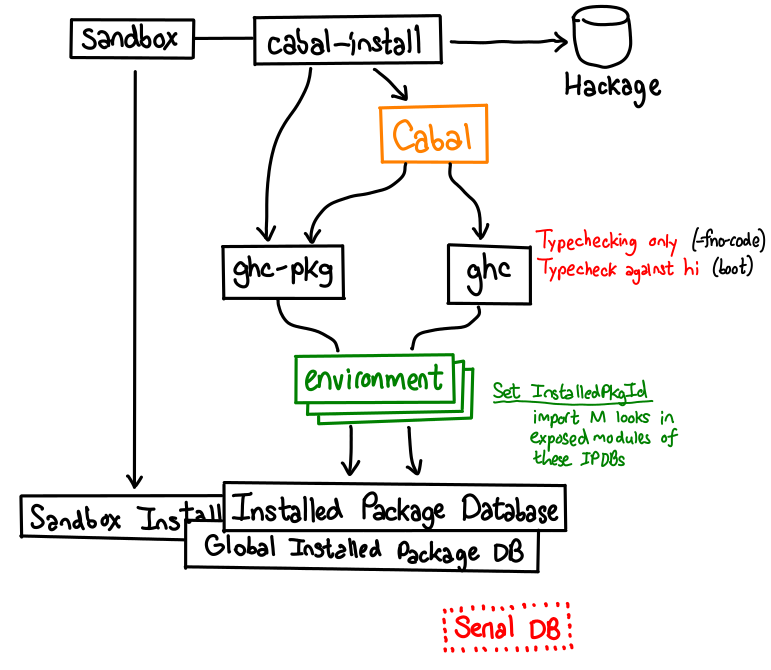
\includegraphics{arch.png}}}
\label{fig:arch}\caption{Architecture of GHC, ghc-pkg and Cabal. Green bits indicate additions from upcoming IHG work, red bits indicate additions from Backpack.  Orange indicates a Haskell library.}
\end{figure}

Here, arrows indicate dependencies from one component to another.
(insert architectural description here)

A particularly important component of this picture is the package
database, sketched in Figure~\ref{fig:pkgdb}.

\begin{figure}[H]
    \center{\scalebox{0.8}{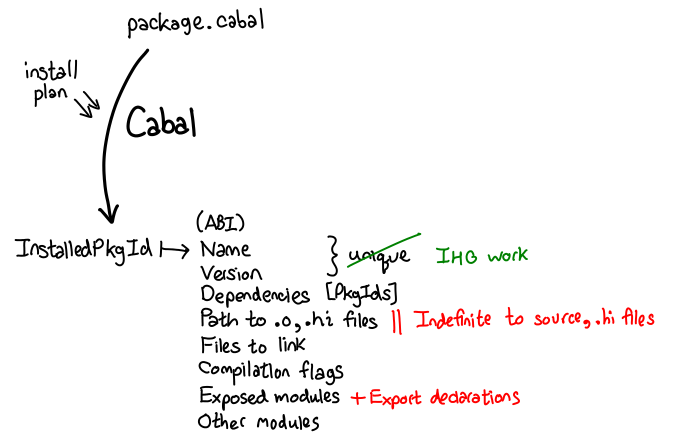
\includegraphics{pkgdb.png}}}
\label{fig:pkgdb}\caption{Anatomy of a package database.}
\end{figure}

An installed package is calculated from a Cabal file through the process
of dependency resolution and compilation.  We can think of it a
database, whose primary key is the InstalledPackageId
(Figure~\ref{fig:current-pkgid}).  This ID uniquely identifies an
instance of an installed package.  The PackageId omits the ABI hash and
is used to qualify linker exported symbols: the current value of this
parameter is communicated to GHC using the \verb|-package-id| flag.

\begin{figure}
    \center{\begin{tabular}{r l}
        PackageId & package name, package version \\
        InstalledPackageId & PackageId, ABI hash \\
    \end{tabular}}
\label{fig:current-pkgid}\caption{Current structure of package identifiers.}
\end{figure}

The database entry itself contains the information from the installed package ID,
as well as information such as what dependencies it was linked against, where
its compiled code and interface files live, its compilation flags, what modules
it exposes, etc.  Much of this information is only relevant to Cabal; GHC
uses a subset of the information in the package database.

In principle, packages with different PackageIds should be linkable
together in the same compiled program, whereas packages with the same
PackageId are not (even if they have different InstalledPackageIds).  In
practice, GHC is currently only able to select one version of a package,
as it clears out all old versions of the package in
\ghcfile{compiler/main/Package.lhs}:applyPackageFlag.

\section{Goals}

There are actually a number of different goals we have for modifying the
packaging system.

\begin{itemize}
    \item Support multiple instances of containers-2.9 \emph{in the
        package database}.  These instances may be compiled against
        different dependencies, have the same dependencies but different
        source files (as when a package is being developed), or be
        compiled with different options.  It is less important to allow
        these instances to be linkable together.

    \item Some easy-to-implement subset of the functionality provided by
        packages with holes (Backpack proper).  This includes support
        of linking an executable containing multiple packages with the
        same package name but different PackageIds.
\end{itemize}

A lower priority goal is to actually allow multiple instances of
containers-2.9 to be linked together in the same executable
program.\footnote{In particular, this requires changes to how linker symbols
are assigned. However, this feature is important to implement a number
of Backpack features.}

A \emph{non-goal} is to allow users to upgrade upstream libraries
without recompiling downstream. This is an ABI concern and we're not
going to worry about it.

\section{Aside: Recent IHG work}\label{sec:ihg}

The IHG project has allocated some funds to relax the package instance
constraint in the package database, so that multiple instances can be
stored, but now the user of GHC must explicitly list package-IDs to be
linked against.  In the far future, it would be expected that tools like
Cabal automatically handle instance selection among a large number of
instances, but this is subtle and so this work is only to do some
foundational work, allowing a package database to optionally relax the
unique package-version requirement, and utilize environment files to
select which packages should be used.  See Duncan's email for more
details on the proposal.

For the purpose of Backpack, the only relevant part of this proposal
is the relaxation of package databases so that there is no uniqueness
constraint on PackageIds; only InstalledPackageIds are unique.

To implement this:

\begin{enumerate}

    \item Remove the ``removal step'' when registering a package (with a flag)

    \item Check \ghcfile{compiler/main/Packages.lhs}:mkPackagesState to look out for shadowing
      within a database. We believe it already does the right thing, since
      we already need to handle shadowing between the local and global database.

\end{enumerate}

Once these changes are implemented, we can program multiple instances by
using \verb|-hide-all-packages -package-id ...|, even if there is no
high-level tool support.

\section{Adding Backpack to GHC}

Backpack additions are described in red in the architectural diagrams.
The current structure of this section is to describe the additions bottom up.

\subsection{Concrete physical identity = PackageId$^*$ + Module name}\label{sec:ipi}

\begin{figure}
    \center{\begin{tabular}{r l}
        PackageId & hash of ``package name, package version, PackageIds of dependent packages'' \\
        InstalledPackageId & hash of ``PackageId, source code, way, compiler flags'' \\
    \end{tabular}}
\label{fig:proposed-pkgid}\caption{Proposed new structure of package identifiers.}
\end{figure}

In Backpack, there needs to be some mechanism for assigning
\emph{physical module identities} to modules, which are essential for
typechecking Backpack packages, since they let us tell if two types are
equal or not. In the paper, the physical identity was represented as the
package that constructed it as well as some representation of the module
source.  We can simplify this slightly: in current Cabal packages, we
require that modules always be given a package-unique logical name;
thus, physical identities can be simply represented as a PackageId plus
module name. (See \ghcfile{compiler/basicTypes/Module.lhs:Module})

However, with the current representation of PackageIds, this is
insufficient: a package is not just its name, but also the regular
tree representing all of its package dependencies.  Thus, we have
to adjust the representation of a PackageId so that it includes this
regular tree, as seen Figure~\ref{fig:proposed-pkgid}.  Since this
tree in general may be quite long, it needs to be shortened in some way,
such as by hashing.

Fortunately, modulo the changes to PackageId, this coincides with how
GHC internally represents modules, which are a pair of a PackageId and the
logical name.  But see the caveats below.

\paragraph{Relaxing package selection restrictions}  As mentioned
previously, GHC is unable to select multiple packages with the same
package name (but different PackageIds).  This restriction needs to be
lifted.  For backwards compatibility reasons, it's probably better to
not overload \verb|-package-id| but add a new flag, maybe \verb|-force-package-id|.

\paragraph{Linker symbols} As we increase the amount of information in
PackageId, it's important to be careful about the length of these IDs,
as they are used for exported linker symbols (e.g.
\verb|base_TextziReadziLex_zdwvalDig_info|).  Very long symbol names
hurt compile and link time, object file sizes, GHCi startup time,
dynamic linking, and make gdb hard to use.  As such, the current plan is
to do away with full package names and versions, and instead use just a
base-62 encoded hash, perhaps with the first four characters of the package
name for user-friendliness.

\paragraph{The ABI hash} Currently, InstalledPackageId
is constructed of a package, version and ABI hash
(generateRegistrationInfo in
\ghcfile{libraries/Cabal/Cabal/Distribution/Simple/Register.hs}).  The
use of an ABI hash is a bit of GHC-specific hack introduced in 2009,
intended to make sure these installed package IDs are unique.  While
this is quite clever, using the ABI is actually a bit inflexible, as one
might reasonably want to have multiple copies of a package with the same
ABI but different source code changes.\footnote{In practice, our ABIs
are so unstable that it doesn't really matter.}

In Figure~\ref{fig:proposed-pkgid}, there is an alternate logical
representation of InstalledPackageId which attempts to extricate the
notion of ABI compatibility from what actually might uniquely identify a
package beyond its PackageId.  We imagine these components to be:

\begin{itemize}
    \item A hash of the source code (so one can register different
        in-development versions without having to bump the version
        number);
    \item Compilation way (profiling? dynamic?)
    \item Compilation flags (such as compilation way, optimization,
        profiling settings)\footnote{This is a little undefined on a package bases, because in principle the flags could be varied on a per-file basis. More likely this will be approximated against the relevant fields in the Cabal file as well as arguments passed to Cabal.};
\end{itemize}

A historical note: in the 2012 GSoC project to allow multiple instances
of a package to be installed at the same time, use of \emph{random
numbers} was used to workaround the inability to get an ABI early
enough.  We are not using this plan.

\paragraph{Wired-in names} One annoying thing to remember is that GHC
has wired-in names, which refer to packages without any version.  A
suggested approach is to have a fixed table from these wired names to
package IDs.

\paragraph{Free variables (or, what is a non-concrete physical
identity?)} Physical identities in their full generality are permitted
to have free variables, which represent holes.  Handling this is a
tricky question, and we defer it to Section~\ref{sec:variables}, when
we talk about packages with holes.

\subsection{Exposed modules should allow external modules}\label{sec:reexport}

In Backpack, the definition of a package consists of a logical context,
which maps logical module names to physical module names.  These do not
necessarily coincide, since some physical modules may have been defined
in other packages and mixed into this package.  This mapping specifies
what modules other packages including this package can access.
However, in the current installed package database, we have exposed-modules which
specify what modules are accessible, but we assume that the current
package is responsible for providing these modules.

To implement Backpack, we have to extend this exposed-modules (``Export declarations''
on Figure~\ref{fig:pkgdb}).  Rather
than a list of logical module names, we provide a new list of tuples:
the exported logical module name and original physical module name (this
is in two parts: the InstalledPackageId and the original module name).
For example, an traditional module export is simply (Name, my-pkg-id, Name);
a renamed module is (NewName, my-pkg-id, OldName), and an external module
is (Name, external-pkg-id, Name).

\subsection{Indefinite packages}\label{sec:indefinite-packages}

In Backpack, some packages still have holes in them, to be linked in
later.  GHC cannot compile these packages, but we still need to install
the interface files in case other packages include them and then perform
type-checking.  Furthermore, we eventually will need to compile them
(once some downstream package links it against its dependencies.)

It seems clear that we need to install packages which do not contain
compiled code, but have all of the ingredients necessary to compile them.
We imagine that instead of providing path to object files, an \emph{indefinite
package} which contains just interface files as well as source. (Figure~\ref{fig:pkgdb})

Creating and typechecking single instances of indefinite packages\footnote{Perhaps we should call them incomplete packages or abstract packages, to line up with previous terminology.} seems to
be unproblematic: GHC can already just type-check code (without compiling it),
and we can also type-check against an interface file, which is currently used for
the recursive module, hs-boot mechanism. (Figure~\ref{fig:arch})

When we need to compile an indefinite package (since all of its
dependencies have been found), things get a bit knotty.  In particular,
there seem to be two implementation paths for this compilation: one path
closer to how GHC compilation currently works, and another which is
conceptually closer to the Backpack formalism.  Here is a very simple
example to consider for both cases:

\begin{verbatim}
package pkg-a where
    A = ...
package pgk-b where -- indefinite package
    A :: ...
    B = [ b = ... ]
package pkg-c where
    include pkg-a
    include pkg-b
\end{verbatim}

\paragraph{The ``downstream'' proposal}  At some point, a package which
relies on an indefinite package fills in all of its dependencies, so
that it can be compiled.  Compilation proceeds by treating all of the
uncompiled indefinite packages as part of a single package: the current
package.  We maintain the invariant that any code generated will export
symbols under the current package's namespace.  So the identifier
\verb|b| in the example becomes a symbol \verb|pkg-c_pkg-b_B_b| rather
than \verb|pkg-b_B_b| (package subqualification is necessary because
package C may define its own B module after thinning out the import.)

One big problem with this proposal is that it doesn't implement applicative
semantics.  If there is another package:

\begin{verbatim}
package pkg-d where
    include pkg-a
    include pkg-b
\end{verbatim}

this will generate its own instance of B, even though it should be the same
as C.  Simon was willing to entertain the idea that, well, as long as the
type-checker is able to figure out they are the same, then it might be OK
if we accidentally generate two copies of the code (provided they actually
are the same).

\paragraph{The ``upstream'' proposal}  Instead of treating all
uncompiled indefinite packages as a single package, each fully linked
package is now considered an instance of the original indefinite
package, except its dependencies are filled in.  Each of these packages
would have different PackageIds, since their dependencies are different
in each case.

While this is conceptually closer to the Backpack model, it is further
away from our current model of compilation: to compile one of these packages,
one essentially has to compile multiple packages, a task previously left
to Cabal.  Fortunately, with the ability to store multiple instances in the database,
it should be possible to place these intermediate results in the database (but
not expose them), and leave it up to the user to decide what to do with the
final package.

\paragraph{Source tarball or preprocessed source?}  Another design choice
to be made is what the representation of the source that is saved is.  There
are a number of possible choices:

\begin{itemize}
    \item The original tarballs downloaded from Hackage,
    \item Preprocessed source files,
    \item Some sort of internal, type-checked representation of Haskell code (maybe the output of the desugarer).
\end{itemize}

Storing the tarballs is the simplest and most straightforward mechanism,
but we will have to be very certain that we can recompile the module
later in precisely the same we compiled it originally, to ensure the hi
files match up (fortunately, it should be simple to perform an optional
sanity check before proceeding.) The appeal of saving preprocessed
source, or even the IRs, is that this is conceptually this is exactly
what an indefinite package is: we have paused the compilation process
partway, intending to finish it later. It allows us to reuse the work
done preprocessing or typechecking.  However, it may be the case that
these phases work differently once library dependencies are known; typechecking
especially, see Section~\ref{sec:variables}.

\section{Module variables and original names}\label{sec:variables}

In Backpack, the physical identities of modules are in fact trees of
variables, constructors and recursive module identities.  As we
mentioned in Section~\ref{sec:ipi}, for concrete modules where there are
no free variables, physical identity maps nicely to an original name.
For packages with holes, the original names mechanism needs to be more
flexible.

The direct approach is to replace original names with Backpack's
physical identities and use unification to do comparisons.  However,
this would require extremely invasive changes to all aspects of GHC, as
the original names assumption is baked quite deeply into the compiler:
we'd like to avoid upsetting this applecart if possible.

One key insight is that when we can only compile when all of the holes
are eliminated; thus all parts of the compilation pipeline beyond
typechecking can, in fact, assume that they will only be dealing with
concrete module identities.  One interpretation of this fact is that
we might actually be able to implement unification properly.

This gives us more latitude for how to
deal with the identities during typechecking: we may, for example,
adopt a conservative analysis (or an optional, dangerously liberal one),
secure in the knowledge that when we compile the final concrete module,
we will typecheck again with everything put together properly.

The next subsection describes one proposal for dealing with this issue,
and in what ways it is unsound.  We imagine there are other strategies

\subsection{Holes have physical module identities associated with definition site}

When compiling a module with a hole, we create a set of interface files
from the signature.  In the current architecture of GHC, we implicitly
assume that all interface files are associated with an \emph{original
name} (see below); thus, this means that it is very natural to assign an
original name to every hole.  If we have a signature package:

\begin{verbatim}
package foo-1x-sig where
    Foo :: ...
\end{verbatim}

Then the physical identity associated with Foo would be
\verb|foo-1x-sig_Foo| (rather than a fresh module variable $\alpha$).

This has implications for signature linking. Take this example from
Section 2.3 of the Backpack paper:

\begin{verbatim}
package yourlib where
    Prelude :: [data List a = ...]
    Yours :: [import Prelude; ...]

package mylib where
    Prelude :: [data Bool = ...]
    include yourlib
    Mine = [import Prelude; import Yours; ...]
\end{verbatim}

The first order of business is that we have to merge the interfaces of
the two Prelude holes, which are associated with different generated
physical identities (\verb|yourlib_Prelude| and \verb|mylib_Prelude|),
and furthermore, \emph{assign an original name to it}.  If we pick,
for example, \verb|mylib_Prelude|, none of the types defined in \verb|yourlib|
will unify in \verb|Mine|; thus, we would need to rename the original names
in \verb|yourlib|.\footnote{Edward: I don't think this is really the
right way to talk about this: Backpack requires a shaping pass and we should
be talking about it}

\iffalse%

% ezyang: So, I thought I knew what I was talking about here, but actually
% the text here needs to be put in the context of shaping, so I need to
% think about this some more

\paragraph{Instantiation and reuse}

If we only ever linked any written signature with a signle implementation, this would actually
be great: when it is time to properly compile a module with holes, we
type check against the true original name of the new module (and just
do a consistency check between the signature and the implementation, modulo
differences in the physical identity)---a case of typechecking proceeding
differently between the initial typecheck and final compilation.

However, conflating a variable with an original name is very bad business.
Consider the graph library 

However, Backpack supports the linking of two signatures together, which
now presents a formidable difficulty: the original names of these two
signatures now must be identified.  Here is a real-world example where
this shows up:

\begin{verbatim}
package foo-1x-sig where
    Foo :: ...

package foo-2x-sig where
    include foo-1x-sig
    Foo :: ...

package foo-2.1 where
    include foo-2x-sig
    Foo = ...

package A where
    include foo-1x-sig
    A = ...

package B where
    include foo-2x-sig
    B = ...

package C where
    include A
    include B
    C = ...

package D where
    include C
    include foo-2.1
\end{verbatim}

Here, we have two signatures for the \verb|foo| library, one of which
is a subset of another (but they are ostensibly backwards compatible).
Package A only uses the 1.x interface, but package B uses the 2.x interface.
Package C uses both of these packages (and implicitly links the two signatures
together), and package D finally links in an actual implementation of the
library.



However, directly modifying original names in this fashion
is likely to be too invasive of a change, since the current compiler has
the assumption that original names can always be checked for equality
is deeply wired in.

Aliasing of signatures means that it is no longer the case that
original name means type equality.  We were not able to convince
Simon of any satisfactory resolution.  Strawman proposal is to
extending original names to also be variables probably won't work
because it is so deeply wired, but it's difficult to construct hi
files so that everything works out (quadratic).


There are some problems with respect to what occurs when two
distinct signatures are linked together (aliasing), we talk these problems in
Section~\ref{sec:open-questions}.

\fi

\subsection{Original names} Original names are an important design pattern
in GHC\@.
Sometimes, a name can be exposed in an hi file even if its module
wasn't exposed. Here is an example (compiled in package R):

\begin{verbatim}
module X where
    import Internal (f)
    g = f

module Internal where
    import Internal.Total (f)
\end{verbatim}

Then in X.hi:

\begin{verbatim}
g = <R.id, Internal.Total, f> (this is the original name)
\end{verbatim}

(The reason we refer to the package as R.id is because it's the
full package ID, and not just R).

How might internal names work with Backpack?

\begin{verbatim}
package P where
    M = ...
    N = ...
package Q (M, R, T)
    include P (N -> R)
    T = ...
\end{verbatim}

And now if we look at Q\@:

\begin{verbatim}
exposed-modules:
        M -> <P.id, M>
        R -> <P.id, N>
        T -> <Q.id, T>
\end{verbatim}

When we compile Q, and the interface file gets generated, we have
to generate identifiers for each of the exposed modules.  These should
be calculated to directly refer to the ``original name'' of each them;
so for example M and R point directly to package P, but they also
include the original name they had in the original definition.


\section{Open questions}\label{sec:open-questions}

Here are open problems about the implementation which still require
hashing out.

\begin{itemize}
    \item Aliasing of signatures means that it is no longer the case that
      original name means type equality.  We were not able to convince
      Simon of any satisfactory resolution.  Strawman proposal is to
      extending original names to also be variables probably won't work
      because it is so deeply wired, but it's difficult to construct hi
      files so that everything works out (quadratic).

  \item Relationship between linker names and InstalledPackageId? The reason
      the obvious thing to do is use all of InstalledPackageId for linker
      name, but this breaks recompilation.  So some of these things
      should go in the linker name, and not others (yes package, yes
      version, yes some compile flags (definitely ways), eventually
      dependency package IDs, what about cabal build flags).  This is
      approximately an ABI hash, but it's computable before compilation.
      This worries Simon because now there are two names, but maybe
      the DB can solve that problem---unfortunately, GHC doesn't ever
      register during compilation; only later.

        Simon also thought we should use shorter names for linker
        names and InstallPkgIds.  This appears to be orthogonal.

    \item In this example:

\begin{verbatim}
    package A where
        A = ...
    package A2 where
        A2 = ...
    package B (B)
        A :: ...
        B = ...
    package C where
        include A
        include B
    package D where
        include A
        include B
    package E where
        include C (B as CB)
        include D (B as DB)
\end{verbatim}

      Do the seperate instantiations of B exist as seperate artifacts
      in the database, or do they get constructed on the fly by
      definite packages which include them?  The former is conceptually
      nicer (identity of types work, closer to Backpack semantics), but
      the latter is easier for linker names. (Simon's first inclination
      is to construct it on the fly.)

      There was another example, showing that we need to solve this
      problem even for indefinite combinations of indefinite modules.
      You can get to it by modifying the earlier example so that C and
      D still have holes, which E does not fill.

  \item We have to store the preprocessed sources for indefinite packages.
      This is hard when we're constructing packages on the fly.

  \item What is the impact on dependency solving in Cabal?  Old questions
      of what to prefer when multiple package-versions are available
      (Cabal originally only needed to solve this between different
      versions of the same package, preferring the oldest version), but
      with signatures, there are more choices.  Should there be a
      complex solver that does all signature solving, or a preprocessing
      step that puts things back into the original Cabal version.
      Authors may want to suggest policy for what packages should actually
      link against signatures (so a crypto library doesn't accidentally
      link against a null cipher package).
      \end{itemize}

\section{Immediate tasks}

At this point in time, it seems we can identify the following set
of non-controversial tasks which can be started immediately.

\begin{itemize}
    \item Relax the package database constraint to allow multiple
        instances of package-version. (Section~\ref{sec:ihg})
    \item Propagate the use of \verb|InstalledPackageId| instead of
        package IDs for typechecking. (Section~\ref{sec:ipi})
    \item Implement export declarations in package format, so
        packages can reexport modules from other packages. (Section~\ref{sec:reexport})
\end{itemize}

The aliasing problem is probably the most important open problem
blocking the rest of the system.

\bibliographystyle{plain}
\bibliography{backpack-impl}

\end{document}
